\section{Architectural Styles and Patterns}

\subsection{Client - Server}
\paragraph{}The application main architecture uses the \textit{client-server} style.
\begin{figure}[H]
	\centering
	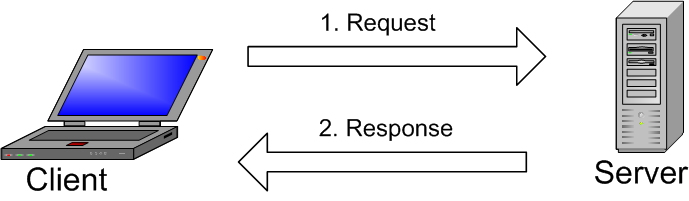
\includegraphics[scale=0.25]{../"Analysis Documents"/client-server}
	\caption{Interactions in a client-server architecture}
\end{figure}
The reasons for this choice are:
\begin{itemize}
	\item The \textit{centrality of the server} and the \textit{sparsity of the clients}: we have different users that need some type of service provided by a particular organization
	\item The \textit{absence of business logic client-side}: our user devices (web browser and mobile applications) must not need to know the back-end logic of the services they are invoking. This ensure scalability and the possibility to add new services or modify the already present with a minimum effort in the update of the applications client side.
\end{itemize}
\paragraph{}The interaction of a client-server system has the client as initiator of the communication, which makes a \textit{request} to the server. The server, received the request, elaborate a \textit{response} using its internal business logic, and finally send it to the client.
\paragraph{}We made the design choice to have \textit{thin} clients, which leads to the following advantages:
\begin{itemize}
	\item The client applications (and of course, the web pages) are easily modifiable
	\item The client applications are power consumption optimized
	\item Easy installation of the app and increased download speed of it (both mobile application and web pages).
\end{itemize}
\subsection{The problem of the notification to the clients}
\paragraph{}A great design issue raised by the requirements of the application is \textit{how the server can contact the clients} (both passengers and taxi drivers). A passenger is contacted by the server when a reservation of him is ready and it was assigned to it a taxi driver. A taxi driver is notified by the server when a request for him is available. We notice immediately that this interaction is basically asynchronous.
\paragraph{} This model of interaction is in conflict with the concept of \textit{client - server} style. \\ Anyway this conflict is only at the modeling level because we can \textit{simulate} this interaction with a low level \textit{polling} policy which uses the client-server paradigm with some optimization in order to minimize the number of requests carried out by the client to the server.
\paragraph{} Anyway the high level architectural style for this kind of interaction is basically a variant of the \textit{publish-subscribe} (event-based).
\paragraph{} From the point of view of implementation there are lots of \textit{messaging frameworks} that can be used: JMS maybe is the most natural choice if we would choose the JEE infrastructure.
\paragraph{} These design choices have been chosen in order to \textit{reduce} the number of request sent by the clients to the server, which are the main drawback of a client-server approach.
\subsection{Three-tier-architecture}
\paragraph{} We decided to use a \textit{three-tier-architecture} for our system.\\
This is simply a specialization of the client-server architecture in which we specify the different layers and components of our system.\\
A schematic representation of this responsibility distribution is at figure \ref{fig:3-tier-architecture}

\begin{figure}[H]
	\centering
	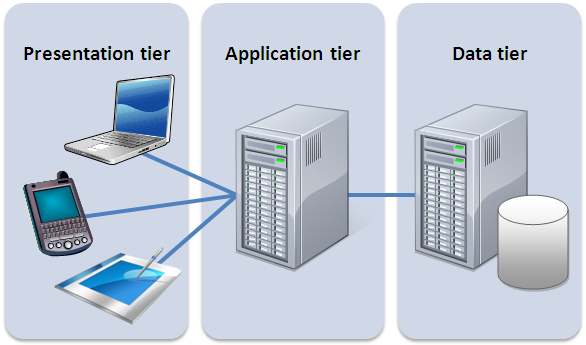
\includegraphics[scale=0.35]{../"Analysis Documents"/3-tier-architecture.png}
	\caption{A representation of a three-tier-architecture}
	\label{fig:3-tier-architecture}
\end{figure}
\paragraph{} So we subdivide our system in three extremely separated layers (or \textit{tiers}):
\begin{itemize}
	\item A \textit{presentation} layer for the graphic rendering of the data and events generated by the system, and from which the end user can interact with the system
	\item An \textit{application} layer entitled to manage all the business logic of the system
	\item A \textit{Data} layer responsible of the storage of informations to be used by the application and presentation layer
\end{itemize}
\paragraph{}The three levels are completely independent and can be replaced easily. In particular, the presentation layer cannot communicate directly with the data tier, but it must forward its requests to the application one, which will use some data access framework to access the database.
\paragraph{} The reasons of this architectural choice are:
\begin{itemize}
	\item The possibility of use \textit{well-defined interfaces} between the different layers. Each layer is dependent uniquely on the interfaces with the other elements of the system. This ensure scalability and, from the data layer side, the possibility of replication and clouding of the resources.
	\item This subdivision of roles makes the defining of the required \textit{programmatic interface} easier. Each layer and each subcomponent will expose an interface which can be part of an API to be used by the future developers in order to improve the services and create new ones.
\end{itemize}


